\documentclass[openacc]{rsproca_new}

% Type of article
\jname{rspa} 
\Journal{Proc R Soc A\ }
\titlehead{Research}

% Packages
\usepackage{mathtools}

% Custom commands
\newcommand{\dd}{\mathrm{d}}
\newcommand{\Var}{\operatorname{Var}}
\newcommand{\Cov}{\operatorname{Cov}}
\newcommand{\Corr}{\operatorname{Corr}}
\newcommand{\Ai}{\operatorname{Ai}}
\newcommand{\Bi}{\operatorname{Bi}}
\newcommand{\E}{\mathbb{E}}
\DeclareMathOperator*{\argmax}{\arg\,max}
\DeclareMathOperator*{\argmin}{\arg\,min}

% Corrections to previously written text are typeset in red.
\newcommand{\edit}[1]{\textcolor{red}{#1}}

%%%%%%%%%%%%%%%%%%%%%%%%%%%%%%%%%%%%%%%%%
%               Main text               % 
%%%%%%%%%%%%%%%%%%%%%%%%%%%%%%%%%%%%%%%%%

\begin{document}

\title{Forecasting tipping times from data}

\author{Davide Papapicco$^{1}$, Lauren Smith$^{1}$ and Graham Donovan$^{1}$}
\address{$^{1}$Department of Mathematics, University of Auckland, New Zealand}
\corres{Graham Donovan\\ \email{g.donovan@auckland.ac.nz}}

\subject{applied mathematics, differential equations, statistical physics}
\keywords{early warning signals, tipping points, numerical methods, statistical inference, multiscale dynamics}

\begin{abstract}
        We combine established results in nonautonomous dynamics, stochastic processes and statistical estimation for stochastic differential equations to derive a fully data-driven pipeline for the accurate forecast of tipping times in complex systems. 
        Our aim is to provide a practical guide for the generation and collection of data to scientists and modelers that are interested in predicting tipping events from recorded timeseries of their systems.
        This pipeline relies on a series of assumptions, discussed and proved throughout this paper, that form an optimal observation protocol for the forecast of tipping times.
        \absbreak 
\end{abstract}

%\rsbreak

\begin{fmtext}
        \section{Introduction}
        Tipping phenomena (or critical transitions) are abrupt changes in the state of complex systems that correspond to disruptive, possibly permanent alterations in their long--term behaviour.
        They have been studied across a heterogenous collection of very different natural and human critical phenomena including ecosystems degradation \cite{OSullivan2023,Kumar2026}, neurobiological activity spikes \cite{Boerner2024}, onset of asthma \cite{Donovan2015}, weakining of ocean currents \cite{Boers2021,Dijkstra2026}, hysteresis in laser systems \cite{Hohl1995}, generation of instabilities in magnetically confined plasma \cite{Cowley2015}, vessels capsizing \cite{Shao2026}, formation of traffic congenstions \cite{Chattopadhyay2026} and civilization collapse \cite{Scheffer2021,Doak2026}.

        The mathematical characterization of such catastrophic events follows the loss of stability of the nonlinear and noisy response of state variables and observables of the system under investigation to slow--varying external forcing.
        A canonical classification of the causes leading to these events has been proposed in \cite{Ashwin2012} distinguishing the cases of bifurcation--induced (B-), rate--induced (R-) and noise--induced (N-) tipping points.
        Furthermore, slow--fast dynamics and bifurcation theory have been shown to provide a modeling framework for the forecast of critical transitions in \cite{Kuehn2011}.
\end{fmtext}

\maketitle

%\section{Introduction}
\noindent
The early prediction of approaching catastrophes, commonly known as \emph{early-warning signals}, relies on the detection of precusors signature from non--stationary 
timeseries such as \emph{critical slowing down} \cite{Tredicce2004}.
        These precursors are often associated to changing statistical quantities, such as sample autocorrelation and variance, to measure the increase in memory of the observed signal.

Several early-warning signals have been proposed in the last two decades; we refer interested readers to \cite{Boettiger2013}, and more recently \cite{Dakos2024}, for a concised overview on the state--of--the--art research on the topic.
Debates regarding the legitimacy of theoretical early-warnings applied to real--worl data have since followed \cite{Ditlevsen2010,Dakos2015} suggesting that caution should be exercised when relying on these indicators to preict critical events \cite{Morr2024a,Parry2026}.
Among the raised concerns, of particular importance for applications are:
\begin{itemize}
  \item recording optimal observables from high--dimensional (spatio--temporal or networked) systems is necessary in order to detect critical slowing down \cite{Lohmann2025b};
  \item reliable and skillfull early-warnings require sufficient timescale separation between the fast (state) and the slow (forcing) variables \cite{Pavithran2021};
  \item predictions based on ensemble averages without uncertainty quantification of the single realizations can lead to missed warnings (i.e. false negatives) and/or spurious signals (i.e. false positives) \cite{Ashwin2025};
  \item lack of knowledge of baseline values of classical early-warning signals result in lack of interpretability of statistical quanties without context and historical trends \cite{Papapicco2026}.
\end{itemize}

In this manuscript we are concerned with the problem of forecasting the time at which complex systems will undergo critical transitions given past and present data.
The forecast is a (linear) extrapolation of the estimated return rate of nonlinear systems slowly ramped towards a saddle-node bifurcation.
Saddle-node B-tipping events are generic across the many applications mentioned above in which the collected timeseries samples provide a discrete time approximation of a slow passage through the tipping point \cite{Tsai2025}.
This paper provides a data--driven pipeline and an observation protocol with which scientists and modelers can collect data to predict such tipping events, far enough in the future and with sufficient accuracy, to enable policies that stop or reverse the catastrophe.

To achive this we leverage well--known results in classical and nonautonomous dynamical systems theory and stochastic dynamics as well as canonical statistical estimation techniques applied to timeseries data.
The pipeline and the protocol rely on a series of assumptions that we discuss and derive; these assumptions provide the constraints that the data must satisfy in order for the forecasting technique to yield consistent and reliable results.

The following discussion is structured as follows.
In \S~\ref{sec:tipping} we introduce the mathematical formalism of tipping times in slow--fast stochastic processes.
In \S~\ref{sec:formulation} we formulate the extrapolation problem at the core of the data--driven pipeline by presenting three techniques to estimate the return rate of a given sample, two of which have already been proposed in the literature and a new one which we introduce.
In \S~\ref{sec:observation} we derive the observation protocoal, that is a series of conditions that allow for the accurate forecast of tipping times from collected measurements or experimental data.
In \S~\ref{sec:application} we apply the proposed methodology to simulated and real--world timeseries data.
In \S~\ref{sec:conclusion} we discuss our findings, address the limitations of the pipeline within the protocol and suggest future directions for this line of research.

\section{Tipping time of a slowly ramped systems}\label{sec:tipping}
The prototypical case of critical transitions in complex system is that of a dynamic saddle-node normal form, with slow (linear) passage through the bifurcation and (additive) noisy fluctuations modelled as an It\^o stochastic differential equation of the form
%
\begin{equation}\label{eq:model}
\dd X_t=f\bigl(X_t,\mu(t)\bigr)\,\dd t+\sigma\,\dd W_t,
\qquad
f(x,\mu):=-\mu-x^2,
\qquad
\mu(t):=\mu_0+\varepsilon t ,
\end{equation}
%
where $X_t\in\mathbb R$ is the state of the system, perturbed by a Wiener process $W_t$ with noise amplitude $\sigma>0$, and $\mu(t)$ is the bifurcation parameter, ramped with constant speed $\varepsilon>0$ from an initial value $\mu_0<0$.
The drift term $f(x,\mu)$ in \eqref{eq:model} has two equilibria $x_{\pm}(\mu)=\pm\sqrt{-\mu}$ for any $\mu<0$; at $\mu=0$ the two branches collide $x_+(0)=x_-(0)=0$ in a saddle-node bifurcation and for $\mu>0$ they annihilate each other.
Small perturbations around the stable equilibrium $x_+(\mu)$ decay exponentially fast at a rate dictated by the leading eigenvalue of the linearized vector field
%
\begin{equation}\label{eq:eigenvalue}
        \lambda(\mu)\coloneqq\partial_xf(x_+(\mu),\mu)=-2\sqrt{-\mu}<0 , \quad \mu<0 .
\end{equation}
%
Specifically, the quantity $1/|\lambda|$ identifies the \emph{correlation} or \emph{relaxation time} of noisy fluctuations towards $x_+(\mu)$.
Evidently, $|\lambda|\downarrow0$ as $\mu\uparrow0$, which in turn gives asymptotically longer relaxation time and eventually the blow-up $1/|\lambda|\to\infty$; this phenomenon is known as \emph{critical slowing down}.
This behaviour is generic for any complex system close enough to a saddle-node bifurcation as the nonlinear dynamics is reduced to the normal form \eqref{eq:model} by a smooth change in coordinates.

For a given ramp speed $\varepsilon>0$, the time at which the leading eigenvalue \eqref{eq:eigenvalue} vanishes corresponds to the time at which the forcing parameter $\mu(t)$ reaches the saddle-node bifurcation $\mu(t)=0$, which is $\tau\coloneqq-\mu_0/\varepsilon>0$.
One can thus rewrite the linear ramp of the forcing parameter to be independent of the initial condition $\mu_0<0$ and parametrized by the time horizon $\tau$ at which the saddle-node bifurcation is reached, i.e.
%
\begin{equation}\label{eq:breaking_time}
        \mu(t) = \mu_0 + \varepsilon t = \varepsilon(t-\tau)<0\quad\forall t<\tau .
\end{equation}
%
Substituting \eqref{eq:breaking_time} in \eqref{eq:eigenvalue} gives an explicit time dependence of the approach to the bifurcation
%
\begin{equation}\label{eq:eigenvalue_time}
        \lambda(t) = -2\sqrt{\varepsilon(\tau-t)}\uparrow0 ,\quad t\uparrow\tau .
\end{equation}

\subsection{Deterministic tipping time}\label{subsec:delay}
Let us first consider the deterministic limit $\sigma\downarrow0$ for which the nonautonomous system \eqref{eq:model} is known as the \emph{dynamic} saddle-node normal form \cite{Berglund2006}.
The time horizon $\tau$ (henceforth \emph{breaking time}) identifies the loss of hyperbolicity of the stable equilibrium branch $x_+(t)\coloneqq x_+(\mu(t))$ as per \eqref{eq:eigenvalue_time}.
In the nonautonomous regime however, the classic notion of $x_+(t)$ is replaced by the pullback attractor $x_{\mathrm{pb}}(t)$ which is the unique solution of \eqref{eq:model} (in the absence of noise $\sigma=0$) satisfying 
%
\begin{equation}\label{eq:pb_attractor}
  \lim_{t\to-\infty}|x_{\mathrm{pb}}(t)-x_+(\mu(t))|=0 .
\end{equation}
%
For a slow passage through the saddle-node bifurcation, i.e. $0<\varepsilon\ll1$, provided that $\mu_0=\lim_{t\to-\infty}\mu(t)\ll0$, the pullback attractor converges to a slow manifold \cite[Thm.~$2.1.7$]{Berglund2006}, which tracks the stable equilibrium branch $x_+(\mu(t))$.
Specifically, the $x_{\mathrm{pb}}(t)$ solution of \eqref{eq:model} lags behind the drift of the \emph{quasi-stationary equilibrium} $x_+(t)$ and persists past the breaking time $\tau$ for some time before blowing-up to $-\infty$.
The trajectory of a slow passage through a saddle-node will thus undergo a bifurcation-induced critical transition at a delayed time $\tau_\mathrm{pb}>\tau$ (henceforth \emph{tipping time}), creating a window of opportunity $\Delta\tau\coloneqq\tau_{\mathrm{pb}}-\tau>0$ to reverse the forcing $\varepsilon$ and avoid the catastrophic dynamical saddle-node.

To quantify the tipping time, and thus identify the window of opportunity, we follow the procedure outlined in \cite{Li2019}.
We start by writing the dynamic saddle-node normal form as a Riccati equation
%
\begin{equation}\label{eq:riccati}
        \frac{\dd x}{\dd t} = f(x,\mu(t)) = \sum_{k=0}^{2}c_k(t)x^k,
\end{equation}
%
with $c_0(t)=\varepsilon(\tau - t)$, $c_1(t)=0$ and $c_2(t)=-1$, and convert it into a second-order, linear system via change of variables $x\mapsto -(c_2(t)y)^{-1}(\dd y/\dd t)$
%
\begin{equation}\label{eq:converted}
        \frac{\dd^2y}{\dd t^2} = c_0(t)y.
\end{equation}
%
Then we can rewrite \eqref{eq:converted} in the rescaled time $s\coloneqq \varepsilon^{1/3}(\tau -t)$ so that it reads as a Airy equation of the form
%
\begin{equation}\label{eq:airy}
        \frac{\dd^2y}{\dd s^2} = sy,
\end{equation}
%
whose general solution is a linear combination of Airy functions of the first $\Ai(s)$ and second kind $\Bi(s)$ \cite[\S~$10.4$]{Abramowitz1965}.
By backward substitution, and in the past limit $t\to-\infty$, the pullback attractor solving \eqref{eq:riccati} is given by
%
\begin{equation}\label{eq:pullback_attractor}
        x_{\mathrm{pb}}(s) = -\varepsilon^{1/3}\frac{1}{\Ai(s)}\frac{\dd\Ai}{\dd s} .
\end{equation}
%
From \eqref{eq:pullback_attractor}, $x_{\mathrm{pb}}\to-\infty$ as $\Ai\to0$, which occurs at $s\approx2.338$.
It thus follows that the tipping time of the pullback attractor is given by $\tau_{\mathrm{pb }}\approx \tau + 2.338\,\varepsilon^{-1/3}$ and the opportunity window scales with the reciprocal of the cubic root of the parameter speed, i.e. $\Delta\tau\propto\varepsilon^{-1/3}$.

\subsection{Tipping time distribution}\label{subsec:exit}
We now consider the more general case of stochastic fluctuations of slow passage through the bifurcation by restoring $\sigma>0$ in \eqref{eq:model}.
As a result, the tipping time $\tau_{\mathrm{pb}}$ is treated as a random variable $\tau_{\mathrm{tip}}$ with an associated probability distribution. 
To characterize $\tau_{\mathrm{pb}}$ for general model of slow-fast stochastic saddle-node normal form we follow the procedures outlined in \cite{Miller2012,Herbert2017}.
To start, consider again the singular limit $\varepsilon\downarrow0$ of \eqref{eq:model}, written as a gradient system 
%
\begin{equation}\label{eq:gradient}
        \dd X_t=-V'\bigl(X_t,\mu\bigr)\,\dd t+\sqrt{2D}\,\dd W_t,
        \qquad
        V(x,\mu):=\mu x + \frac{x^3}{3},    
\end{equation}
%
where $V(x,\mu)$ is the potential of the vector field $f(x,\mu)$ and $D\coloneqq\sigma^2/2$ is the diffusion intensity.
The equilibria $x_{\pm}(\mu)=\pm\sqrt{-\mu}$ of $f$ correspond to the stationary points of $V$, respectively its local minimum and local maximum.
At any $\mu<0$, the potential barrier, separating the local minimum $x_+(\mu)$ from the local maximum $x_-(\mu)$ is
%
\begin{equation}\label{eq:barrier}
        \Delta V\coloneqq V\bigl(x_-(\mu)\bigr)-V\bigl(x_+(\mu)\bigr) = \frac43(-\mu)^{3/2} .
\end{equation}
%
The critical transition of a solution of \eqref{eq:model}, starting in a neighbourhood of $x_+(\mu)$, can thus be associated to the escape of an overdamped particle across the potential barrier $\Delta V$ driven by noisy fluctuations of intensity $D$.
For fixed values of $\mu<0$ such that $\Delta V\gg D$, these escapes are rare events described by Freidlin--Wentzell theory \cite{Freidlin2012} which has been recently applied in statistical mechanics \cite{Santolin2025}.
In particular, the event of a trajectory $X_t$ of \eqref{eq:gradient}, starting near $x_+(\mu)$ and reaching $x_-(\mu)$ across the potential barrier $\Delta V$, satisfies a so-called \emph{large deviation principle}.
The \emph{first exit time} of such event \cite[\S~$5.5$]{Gardiner2009}  
%
\begin{equation}\label{eq:first_exit}
        \tau_{\mathrm{exit}} \coloneqq \inf\{t\ge0\;:\;X_t\le x_-(\mu)\}, 
\end{equation}
%
is asymptotically exponentially distributed \cite[Thm.~$2.3$]{Berglund2013}
%
\begin{equation}\label{eq:large_deviation_principle}
        \tau_{\mathrm{exit}}\overset{d}{\approx}\exp\bigl(k(\mu)\bigr) , \quad D\downarrow0,
\end{equation}
%
where the rate parameter is given by Kramers formula
%
\begin{equation}\label{eq:rate}
        k(\mu)=\frac{\sqrt{V''\bigl(x_+(\mu)\bigr)\,|V''\bigl(x_-(\mu)\bigr)|}}{2\pi}\,\exp\biggl(-\frac{\Delta V}{D}\biggr)
        =\frac{\sqrt{-\mu}}{\pi}\exp\biggl(-\frac{4(-\mu)^{3/2}}{3D}\biggr).
\end{equation}
%
Notice that the reciprocal of the escape rate in \eqref{eq:rate} gives the \emph{mean first exit time} of \eqref{eq:first_exit}, i.e. $\E[\tau_{\mathrm{exit}}] = 1/k(\mu)$.
This result, originally formulated for stationary diffusion \cite{Day1983} and jump processes \cite{Imkeller2006}, was then extended to the dynamic saddle-node normal form \eqref{eq:model}.
In the limiting regime of low noise intensity $D\ll\varepsilon/2$, the approximate distribution $\tau_{\mathrm{tip}}\overset{d}{\approx}p_1$ of the tipping time $\tau_{\mathrm{tip}}$ has been shown to be \cite[Eq.~$(19)$]{Miller2012}
%
\begin{equation}\label{eq:small_noise}
        p_1(t)\coloneqq\frac{\varepsilon^{2/3}}{\sqrt{4\pi^{5}D}\,\Bi^{2}\bigl(-\mu(t)\varepsilon^{-2/3}\bigr)\,\mathcal J(t)^{1/2}}
        \exp\Biggl[-\frac{\varepsilon^{2/3}\,\Ai^{2}\bigl(-\mu(t)\varepsilon^{-2/3}\bigr)}
        {4\pi^{2}D\,\Bi^{2}\bigl(-\mu(t)\varepsilon^{-2/3}\bigr)\,\mathcal J(t)}\Biggr] ,
\end{equation}
%
with $\mathcal J(t)\coloneqq\int_{-\infty}^{t}\Ai^{4}\bigl(-\mu(s)\varepsilon^{-2/3}\bigr)\,\dd s$. 
We remark that $p_1(t)$ has support in the interval $\tau+1.17 \varepsilon^{-1/3} < t < \tau + 3.27 \varepsilon^{-1/3}$ and it contains the tipping time of the pullback attractor $\tau_{\mathrm{pb}}\approx\tau+2.338\,\varepsilon^{-1/3}$.
Furthermore \eqref{eq:small_noise} is approximately Gaussian locally to its maximum
%
\begin{equation}\label{eq:small_noise_approximation}
        \tau_{\mathrm{tip}}\overset{d}{\approx}\mathcal{N}\biggl(\tau_{\mathrm{pb}}\bigl[1+O(D/\varepsilon)\bigr],O\bigl(D\varepsilon^{-5/3}\bigr)\biggr),
\end{equation}
%
with mean close to the tipping time of the deterministic solution, i.e. $\E[\tau_{\mathrm{tip}}]\approx\tau_{\mathrm{pb}}$
 
In the opposite regime of large noise intensity $\varepsilon/2\ll D$, and up to $-\mu(t)\gg D^{2/3}$, it was later shown that the approximate tipping time distribution $\tau_{\mathrm{tip}}\overset{d}{\approx}p_2$ has a maximum before the breaking time $\tau$ and it has the form \cite[Eq.~$(4)$]{Herbert2017}
%
\begin{equation}\label{eq:large_noise}
        p_2(t)\coloneqq k\bigl(\mu(t)\bigr)\,
        \exp\biggl[-\frac{D}{2\pi\varepsilon}\,
        \exp\biggl(-\frac{\Delta V\bigl(\mu(t)\bigr)}{D}\biggr)\biggr] ,
\end{equation}
%
where $k(\mu(t))$ is the Kramers escape rate given in \eqref{eq:rate} and $\Delta V(\mu(t))$ is the potential barrier given in \eqref{eq:barrier}.

\begin{figure}[t]
    \centering 
    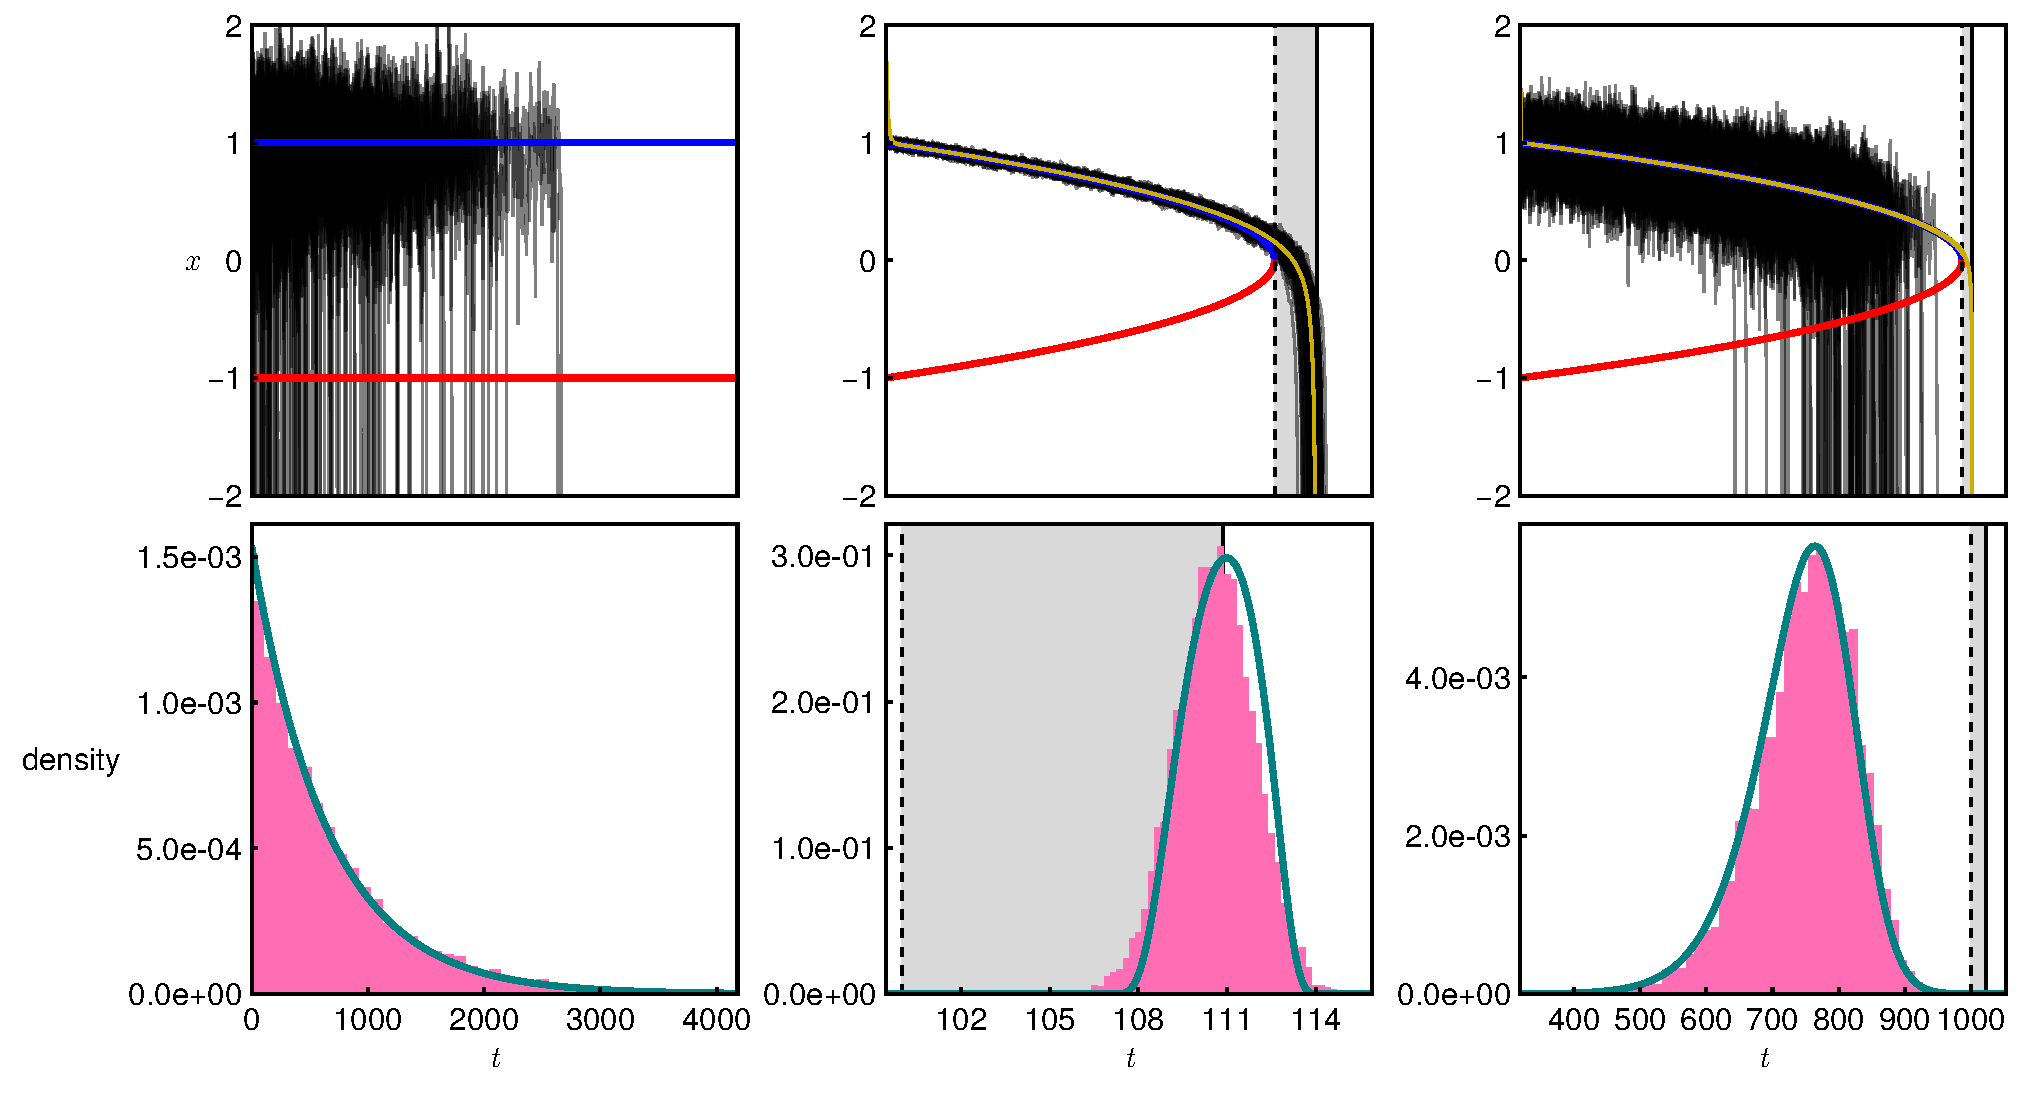
\includegraphics[keepaspectratio, width=\textwidth]{./figures/tipping_times_distribution.pdf}
    \caption{Analytical (teal curves, bottom row) and empirical (pink histograms, bottom row) distribution of the tipping time random variable $\tau_{\mathrm{tip}}$ of $10{,}000$ solutions (black curves, top row) of the saddle-node normal form \eqref{eq:model} from the stable branch $x_+(\mu(t))$ (blue curves, top row) across the unstable branch $x_-(\mu(t))$ (red curves, top row).
             Leftmost column (N-tipping): stationary regime \eqref{eq:large_deviation_principle} with $\mu=-1$ and $D=0.25$.
             Middle column (B-tipping): slow passage through the bifurcation \eqref{eq:small_noise} with $\mu_0=-1$, $\varepsilon=10^{-2}$ and $D=10^{-3}$.
             Rightmost column (N-tipping): early escapes due to large noise \eqref{eq:large_noise} with $\mu_0=-1$, $\varepsilon=10^{-3}$ and $D=0.06$.
             The window of opportunity $\Delta\tau$ (gray shaded band in the middle and rightmost columns) is bounded from below (dashed black lines) by the breaking time $\tau$ and from above (solid black lines) by the tipping time of the pullback attractor $\tau_{\mathrm{pb}}$ (orange curve, top row).
     }
    \label{fig:tipping_times_distribution}
\end{figure}

\section{Forecasting problem}\label{sec:formulation}
From \S~\ref{sec:tipping}, we summarize three important results that motivate the forecasting of tipping times:
%
\begin{enumerate}
        \item for a slow passage through a saddle-node bifurcation the leading eigenvalue $\lambda(t)$ explicitly depends on the breaking time $\tau$ via Eq.~\eqref{eq:eigenvalue_time};
        \item the time at which a slowly ramped solution tips $\tau_{\mathrm{pb}}$ is delayed with respect to the breaking time $\tau$ by a factor of $\varepsilon^{-1/3}$ that depends on the speed of the forcing, thereby creating an opportunity window $\Delta\tau$;
        \item in the small noise regime $\sigma=\sqrt{2D}\ll\sqrt{\varepsilon}$, the delayed tipping time of a noisy solution $\tau_{\mathrm{tip}}$ occurs almost always after the breaking time $\tau$, as per the support of the density $p_1(t)$ in Eq.~\eqref{eq:small_noise}, and on average close to the deterministic tipping time, as per Eq.~\eqref{eq:small_noise_approximation}.
\end{enumerate}
%
Provided a timeseries that is slowly ramped towards a saddle-node bifurcation, with noise $\sigma$ and speed $\varepsilon$ satisftying $0<\sigma^2\ll\varepsilon\ll1$, then, if we accurately forecast the breaking time $\tau$ (i), we identify a window of opportunity (ii) and avoid the bifurcation-induced catastrophe with high probability (iii) by stopping or reversing the forcing of the parameter.
To formulate the forecasting problem of the breaking time $\tau$ we introduce the \emph{(squared) return rate} $\alpha(t)\coloneqq\lambda^2(t)$ which, from \eqref{eq:eigenvalue_time}, reads
%
\begin{equation}\label{eq:return_rate}
        \alpha(t) = 4\varepsilon(\tau-t)>0\quad\forall t<\tau . 
\end{equation}
%
Notice that, while $\alpha(t)\downarrow0$ as $t\uparrow\tau$ just like $-\lambda(t)$, the return rate in \eqref{eq:return_rate} establishes an affine dependence of the return rate on time $t$ which benefits the forecasting of $\tau$ using timeseries data.

To understand this suppose that $\mathcal{X}_1\coloneqq\{X^{(1)}_j\coloneqq X_{t^{(1)}_j}\}_{j=1,\dots,n}$, $t^{(1)}_j<t^{(1)}_{j+1}$, is a solution of \eqref{eq:model} that is at safe distance from the bifurcation, i.e. $t^{(1)}_n\ll\tau$.
Assume also that we can estimate the true return rate \eqref{eq:return_rate} from the sample $\mathcal{X}$, which we denote with $\hat\alpha_1\coloneqq\hat\alpha(t^{(1)}_n)$.
We are then presented with another sample $\mathcal{X}_2$, which is also at safe distance from the bifurcation but closer to it than the previous sample $\mathcal{X}_1$, i.e. $t^{(1)}_n<t^{(2)}_n$; once again, assuming we can do so, we estimate the return rate $\hat\alpha_2$.
Suppose with repeat this procedure for $N$ different samples $\mathcal{X}_1,\dots,\mathcal{X}_N$, yielding a sequence $\hat{\alpha}\coloneqq\{\hat\alpha_j\}_{j=1,\dots,N}$.
Given this sequence $\hat\alpha$ we can then fit a linear model of the form $\hat\alpha(t) = \hat m t + \hat q$, with slope $\hat m$ and intercept $\hat q$. 
The forecasted breaking time $\hat\tau$ thus corresponds to the zero-crossing of the linear fit, which by extrapolation reads $\hat\tau = -\hat q/\hat m$.

Conseqentially, we translated the problem of forecasting the breaking time $\tau$ from timeseries data $\mathcal{X}_1,\dots,\mathcal{X}_N$ into a trivial, linear extrapolation $\hat\tau$ from estimated return rates $\hat\alpha$.
This procedure however features two bottlenecks: first, we need $\hat\alpha$ to be a sequence of unbiased and accurate estimators of the ground truth $\alpha$ and; second, given those estimates $\hat\alpha$, we need the linear extrapolation $\hat\tau=-\hat q/\hat m$ to be as close as possible to the ground truth $\tau$ to not shrink the window of opportunity.
In particular, depending on applications, we would prefer to slightly underestimate the breaking time $\hat\tau\lesssim\tau$, rather than slightly overestimating it $\hat\tau\gtrsim\tau$, thereby biasing our forecast to minimize missed alarms (i.e. false negatives) in favour of spurious warnings (i.e. false positives).
In the remaining of this section we present three data-driven techniques to accurately extract the estimates $\hat\alpha$ from a sample $\mathcal{X}$ while we address the extrapolation problem in \S\ref{sec:observation}.

\subsection{Ornstein-Uhlenbeck approximation}\label{subsec:OUP}
Let us start by characterizing the statistical properties of the noisy fluctuations of a solution $\mathcal{X}$ of \eqref{eq:model} around the pullback attractor $x_{\mathrm{pb}}(t)$ given in Eq.~\eqref{eq:pullback_attractor}.
We write the solution variable as a superposition $X_t\coloneqq x_{\mathrm{pb}}(t)+Z_t$ of a deterministic $x_{\mathrm{pb}}(t)$ and a stochastic component $Z_t$.
Substituting this into \eqref{eq:model}, recalling that by definition $\dd x_{\mathrm{pb}}=f(x_{\mathrm{pb}},\mu)\dd t$, we get
%
\begin{equation}\label{eq:fluctuations}
  \dd Z_t=\bigl(-2 x_{\mathrm{pb}}(t)\,Z_t-Z_t^2\bigr)\dd t+\sigma\,\dd W_t .
\end{equation}
%
At any time $t\ll\tau$ away from the saddle-node bifurcation $f(x_{\mathrm{pb}},\mu)\approx f\bigl(x_+(\mu),\mu\bigr)$ which implies $\partial_x f(x_{\mathrm{pb}},\mu)\approx\lambda(t)$.
Substituting this into \eqref{eq:fluctuations} gives
%
\begin{equation}\label{eq:fluctuations_scaled}
        \dd Z_t=\bigl(\lambda(t)\,Z_t-Z_t^2\bigr)\dd t+\sigma\,\dd W_t .
\end{equation}
%
It can be shown that $|Z_t|\approx\sigma/\sqrt{2|\lambda(t)|}$ \cite[Thm.~$4.1$]{Kuehn2011}, and thus $Z_t^2=o\bigl(|\lambda(t)Z_t|\bigr)$ for any $\sigma\ll\sqrt{\varepsilon}$ and any $t\ll\tau$ such that $\sigma\ll\sqrt{2}\bigl(4\varepsilon(\tau-t)\bigr)^{3/4}$.
We can therefore reasonably approximate \eqref{eq:fluctuations_scaled} by neglecting the nonlinear term $Z_t^2$, thereby obtaining 
%
\begin{equation}\label{eq:oup}
        \dd Z_t\approx\lambda(t)\,Z_t\dd t+\sigma\,\dd W_t .
\end{equation}
%
The linear, nonautonomous Eq.~\eqref{eq:oup} is a time-inhomogeneous Ornstein-Uhlenbeck process.
Suppose the sample $\mathcal{X}$ is recorded across a time window $T_w>0$ in which $\lambda(t)\approx\lambda$ is approximately constant. 
Then such sample can be considered as an approximate solution of the stationary process \eqref{eq:oup} which admits a Gaussian distribution \cite[\S~$3.8$]{Gardiner2009} with zero mean $\E[Z_t]\eqqcolon\bar{Z}=0$ and variance $\Var[Z_t]\eqqcolon\gamma=\sigma^2/2|\lambda|$.
Written in terms of the return rate $\alpha=\lambda^2$, the last identity reads
%
\begin{equation}\label{eq:oup_variance}
        \gamma = \frac{\sigma^2}{2\sqrt{\alpha}} .
\end{equation}
%
Let $\hat\gamma$ be the sample variance of $\mathcal{X}$, then \eqref{eq:oup_variance} gives a sample estimate of the return rate
%
\begin{equation}\label{eq:OUP}
        \hat\alpha = \frac{\sigma^4}{4\hat\gamma^2} .
\end{equation}
%
The use of the sample variance as an early-warning signal dates back to the very first attempts in predicting bifurcation-induced tipping points and it has since been established as a benchmark precursor of critical slowing down (see e.g. \cite{Kuehn2011} and references therein).

\subsection{Autoregressive approximation}\label{subsec:AC1}
In the same time window $T_w>0$ above, the homogeneous Ornstein-Uhlenbeck process has correlation function $\Corr(Y_t,Y_{t+Tw})=\gamma\exp\bigl(-\sqrt{\alpha}T_w\bigr)$ \cite[\S~$3.8$]{Gardiner2009}, with $\gamma$ given in \eqref{eq:oup_variance}.
As a result, the discrete observations in the sample $\mathcal{X}$ can be approximated by fitting a continuous-time autoregressive model of order one
%
\begin{equation}\label{eq:autoregressive}
        X_{j+1}\approx\rho X_{j} + \sqrt{\gamma(1-\rho^2)}\,\eta_t , \quad \eta_t\sim\mathcal{N}(0,1),
\end{equation}
%
where 
%
\begin{equation}\label{eq:ac1}
        \rho\coloneqq\gamma^{-1}\Corr(X_t,X_{t+\Delta}), \quad \Delta=t_{j+1}-t_j, 
\end{equation}
%
is the autocorrelation coefficient at lag$-1$.
Given the sample mean $\hat X$ the sample autocorrelation coefficient can be obtained by maximum likelihood estimation \cite{Sahalia2002} and it reads
%
\begin{equation}\label{eq:ac1_sample}
        \hat\rho = \frac{\sum_{j=1}^{n-1}(X_j - \hat X)(X_{j+1} - \hat X)}{\sum_{j=1}^{n}(X_j - \hat X)^2}.
\end{equation}
%
Using \eqref{eq:ac1_sample} one can estimate the return rate of the sample $\mathcal{X}$ using the autoregressive approximation 
%
\begin{equation}\label{eq:AC1}
        \hat\alpha = \biggl(\frac{\log\hat\rho}{\Delta}\biggr)^2.
\end{equation}
%
Autoregressive based early-warning signals have found widespread applications in ecology \cite{Dakos2012} and climate science \cite{Boers2021}.
In particular, estimators of the form \eqref{eq:AC1} have been used in \cite{Ditlevsen2023} for estimating the tipping time of the subpolar gyre of the Atlantic Meridional Overturning Circulation system, and in \cite{Ashwin2025} for establishing a framework that quantifies the predicting skill of early-warning signals.

\subsection{Euler-Maruyama approximation}\label{subsec:LLS}
A solution of the nonlinear system \eqref{eq:model} in a time window $T_w>0$ as per above, can be approximated by the process \cite[\S~$8.4$]{Lord2014}
%
\begin{equation}\label{eq:EM}
        X_{t+1} = X_t + f(X_t,\mu)\Delta + \sigma\sqrt{\Delta}\,\xi_t , \quad \xi_t\sim\mathcal{N}(0,1) .
\end{equation}
%
The sequence above is the Euler-Maruyama approximation of \eqref{eq:model} and it corresponds to the stochastic generalization of the Euler time-stepping method for ordinary differential equations.
We can rearrange the terms in \eqref{eq:EM} to define the first-order time increments of the Euler-Maruyama approximation
%
\begin{equation}\label{eq:increments}
        Y_t\coloneqq\frac{X_{t+1} - X_t}{\Delta} = f(X_t,\mu) + \tilde{\xi}_t , \quad \tilde{\xi}_t\sim\mathcal{N}\biggl(0,\frac{\sigma^2}{\Delta}\,\biggr) .
\end{equation}
%
Provided a sample $\mathcal{X} = \{X_j\}_{j=1,\dots,n}$ in a time window $T_w=n\Delta$, and a choice of the model function $f$, Eq.~\eqref{eq:increments} can be interpreted as an ordinary least--squares regression problem, with normally distributed residuals $r_j\coloneqq Y_{j+1} - f(X_j)=\tilde{\xi}_t$.
This is part of a broader class of drift inference methods called \emph{quasi-maximum likelihood estimators} \cite{Jimenez2020}.

Away from the saddle-node bifurcation, the sample is approximately an Ornstein-Uhlenbeck process of the form \eqref{eq:oup} and thus we can reasonably fit a linear model of the form $f(x,\theta) = \theta x$ to the time increments $Y_j$.
Substituting this ansatz into \eqref{eq:increments}, and minimizing the square root of the sum of the squared residuals across the sample, yields the optimization problem
%
\begin{equation}\label{eq:ordinary_least_squares}
        \hat\theta = \argmin_{\theta\in\mathbb{R}}\Biggl(\sqrt{\sum_{j=1}^{n-1}\bigl(Y_j-f(X_j,\theta)\bigr)^2}\Biggr) ,
\end{equation}
%
which is linear in $\theta$ due to $f\in\mathbb{P}_1[x]$.
The solution of \eqref{eq:ordinary_least_squares} is given by the normal equation
%
\begin{equation}\label{eq:normal_equation}
        \hat\theta = (A^TA)^{-1}A^TY,
\end{equation}
%
where $Y=(Y_j)_{j=1,\dots,n-1}$ is the vector of observed time increments of the sample $\mathcal{X}$ and $A=(X_j)_{j=1,\dots,n-1}$ is the model vector of the linear fit $f$ to the sample $\mathcal{X}$.
Notice that, by definition, $\hat{\theta}$ is an estimate of the leading eigenvalue $\lambda$ of the underlying nonlinear evolution and thus
%
\begin{equation}\label{eq:LLS}
        \hat\alpha = \hat{\theta}^{\,2},
\end{equation}
%
is a sample estimate of the return rate using an ordinary (linear) least--squares approximation. 
The application of quasi-maximum likelihood estimations for the construction of early-warning signals is much more recent than the more established autoregressive and Ornstein-Uhlenbeck approximation, with an early adoption discussed in \cite{Papapicco2026}.

\section{Observation protocol}\label{sec:observation}
The return rate estimators using the Ornstein--Uhlenbeck \eqref{eq:OUP}, autoregressive \eqref{eq:AC1} and Euler--Maruyama \eqref{eq:LLS} approximations provide three different, data--drive pipelines to extract $\hat\alpha$ from a given sample $\mathcal{X}$ collected over a time window $T_w=n\Delta$, with $n>0$ number of observations sampled at (regular) frequency $\Delta$.
As noted at the beginning of \S~\ref{sec:formulation} however, we then use these estimates to forecast the tipping time $\hat\tau$ given a sequence of samples $\mathcal{X}_1,\dots,\mathcal{X}_N$.
In this section we address this problem in two parts.
First, we discuss the accuracy and uncertainty associated to the estimators of the return rate $\hat\alpha$ proposed above.
Second, we formulate the extrapolation problem of $\hat\tau$ given a sequence $\hat\alpha=\{\hat\alpha_j\}_{j=1,\dots,N}$ of estimators of the return rate and construct the full, data-driven pipeline for the accurate forecasting problem given input timeseries data.

\subsection{Estimating the return rate}\label{subsec:estimators}
The optimal estimation of the return rate from a finite sample is, perhaps unsurprisingly, highly limited by the quality of the input data provided by the samples $\mathcal{X}_1,\dots,\mathcal{X}_N$.
We hereby discuss three major design constraints that modellers and scientists have to consider when applying the proposed forecasting methodology to their samples.

\subsubsection{Admissible time horizon}\label{subsubsec:horizon}
First observe that the analytical return rate \eqref{eq:return_rate}, on which the sample estimators \eqref{eq:OUP}, \eqref{eq:AC1} and \eqref{eq:LLS} are based on, is obtained from the time--dependent eigenvalue \eqref{eq:eigenvalue_time}, which is itself evaluated along the drifting quasi--steady equilibrium $x_+(\mu(t))$.
However, if the sample $\mathcal{X}$ is assumed to be a slowly forced solution of \eqref{eq:model} away from the bifurcation, then it must follow the pullback attractor \eqref{eq:pb_attractor}, which lags behind $x_+(\mu(t))$ at any $t<\tau$.
In the slow regime (after the fast relaxation of the initial condition) the distance at which $x_{\mathrm{pb}}(t)$ tracks $x_+(\mu(t))$ increases with time and it reaches its maximum at the saddle-node bifurcation $|x_{\mathrm{pb}}(t)-x_+(\mu(t))|=O(\varepsilon^{1/3})$, $t\uparrow\tau$ \cite[Thm.~$2.2.2$]{Berglund2006}.
We are thus interested to quantify a time horizon $t=T_c$ for which the return rate $\alpha(t)$ of the quasi-steady equilibrium is accurate, at least to first-order, to that of the pullback attractor $\alpha_{\mathrm{pb}}(t)=\lambda_{\mathrm{pb}}^2(t)=4x_{\mathrm{pb}}^{\,2}(t)$.
Sufficiently far from the saddle-node bifurcation we can exploit the asymptotic expansion of Airy's function \cite[\S~$10.4$]{Abramowitz1965} to approximate \eqref{eq:pullback_attractor} to first-order
%
\begin{equation}\label{eq:asymptotic_pullback_attractor}
  x_{\mathrm{pb}}(s)\approx \varepsilon^{1/3}\biggl(\sqrt{s} + \frac{1}{4s}\biggr) , \quad s=\varepsilon^{1/3}(\tau-t)\to\infty.
\end{equation}
%
In this regime, the return rate for the pullback attractor is thus
%
\begin{equation}\label{eq:pb_return_rate}
  \alpha_{\mathrm{pb}}(t) = \alpha(t) + \frac{1}{4(\tau-t)^2} + 2\sqrt{\frac{\varepsilon}{\tau-t}},
\end{equation}
%
and dividing each term in \eqref{eq:pb_return_rate} by $\alpha(t)$ gives
%
\begin{equation}\label{eq:lag_correction}
  \frac{\alpha_{\mathrm{pb}(t)}}{\alpha(t)} = 1 + \frac{1}{16 \varepsilon(\tau - t)^3} + \frac{1}{2\sqrt{\varepsilon(\tau - t)^3}} = 1 + 2\eta(t) + \eta^2(t) = \bigl(1+\eta(t)\bigr)^2 ,
\end{equation}
%
where $\eta(t)\coloneqq 1/(4\sqrt{\varepsilon(\tau-t)^3})$ quantifies the lag correction of the return rate of the pullback attractor.
From \eqref{eq:lag_correction} it follows that $\alpha(t)\approx \alpha_{\mathrm{pb}}(t)$ at any time $t\ll\tau$ such that $\eta(t)\ll1$, from which we obtain the admissible time horizon
%
\begin{equation}\label{eq:admissible_time_horizon}
  T_c \lesssim\tau - \varepsilon^{-1/3} .
\end{equation}
%
\begin{figure}[t]
    \centering 
    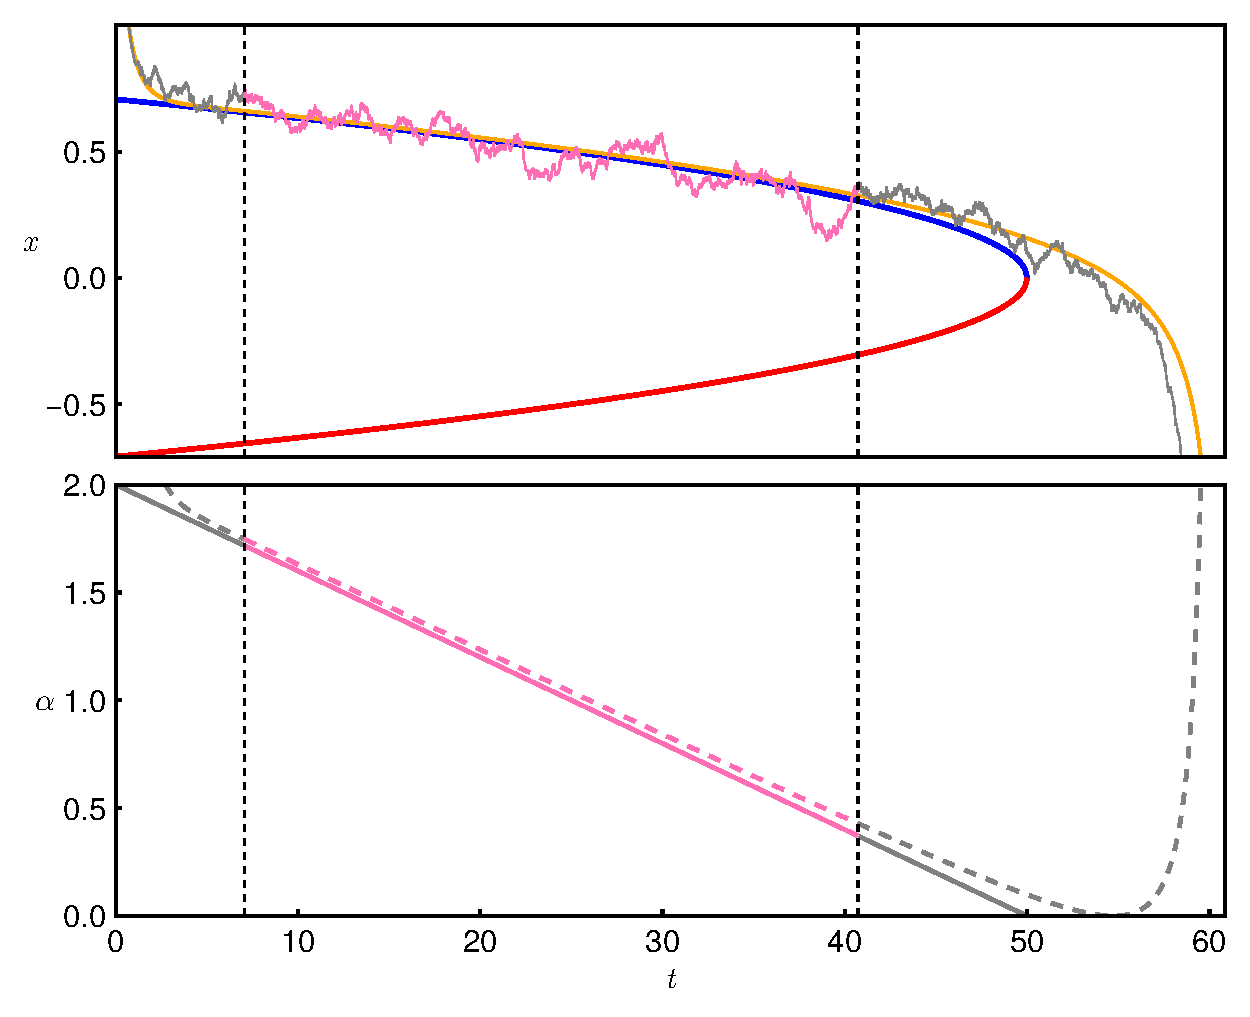
\includegraphics[keepaspectratio, width=\textwidth]{./figures/admissible_time_horizon.pdf}
    \caption{Accuracy of the return rate of quasi-steady equilibrium $\alpha(t)$ (solid pink curve in the bottom plot) with respect to that of the pullback attractor $\alpha_{\mathrm{pb}}(t)$ (dashed pink curve in the bottom plot) for the saddle-node normal form \eqref{eq:model}.
    The solution $\mathcal{X}$ (pink curve in the top plot) follows the pullback attractor $x_{\mathrm{pb}}$ (orange curve) which track the quasi-steady equilibrium $x_+(t)$ (blue curve) with speed $\varepsilon=10^{-2}$ and noisy fluctuations $\sigma=0.6\sqrt{\varepsilon}$.
    The time window in which $\alpha(t)\approx\alpha_{\mathrm{pb}}(t)$ to first order (dashed black lines) is given by the extintion of the transient of the pullback attractor on the lower bound (which here is taken as ten times the relaxation time from the initial condition $x_{\mathrm{pb}}(0)=2$) and by the admissible time horizon \eqref{eq:admissible_time_horizon}.}
    \label{fig:admissible_time_horizon}
\end{figure}
%
The critical threshold \eqref{eq:admissible_time_horizon} gives us a criterion for which the estimation of the frozen return rate yields admissible results for the extrapolation of the tipping time, as the lag correction $\eta(t)$ of the pullback attractor with respect to the quasi-steady equilibrium $x_+(\mu(t))$ is negligible. 

\subsubsection{Biased estimators}\label{subsubsec:effects}
Provided that the sample is in the admissible time horizon $t<T_c$ quantified above, a local estimation of $\alpha(t)$ requires that the sample $\mathcal{X}$ is recorded over a time window $T_w$ in which the leading eigenvalue $\lambda(t)$ at the quasi--steady equilibrium remains approximately constant.
This in turn requires the sample to be limited in a finite observation window $T_w=n\Delta$ that induces biases and uncertainties in the estimation of the return rate.

To quantify those, we shall henceforth adopt an ensemble approach in which $\Omega = \{\mathcal{X}_{j}\}_{j=1,\dots,N}$ denotes a collection of $N>1$ independent and identically distributed finite samples that correspond to different noise realizations of \eqref{eq:model}.
In particular, let us assume that each sample $\mathcal{X}_j$ in the ensemble $\Omega$ is a sequence of stationary residuals obtained by detrending a finite windowed solution of \eqref{eq:model} so that $t^{(1)}_n\equiv t^{(N)}_n$.
Then, the resulting Ornstein-Uhlenbeck processes \eqref{eq:oup} can be approximated by order one autoregressive models of the form \eqref{eq:autoregressive}.

Then let $\hat \beta$ be a generic random variable estimating some ground truth $\beta$ from a single sample in the ensemble.
Denote $\E[\hat \beta]$ to be the ensemble mean of $\hat\beta$ over $\Omega$ and $\Var[\hat\beta]$ to be the variance of $\hat\beta$ over the ensemble $\Omega$.
We thus define the bias $b_{\hat\beta}$ and uncertainty $u_{\hat\beta}$ of the estimator $\hat\beta$ in the canonical fashion
%
\begin{equation}\label{eq:bias_and_uncertainty}
  b_{\hat\beta}\coloneqq\E[\hat\beta - \beta] \quad \text{and}\quad u_{\hat\beta}\coloneqq\sqrt{\Var[\hat\beta]} ,
\end{equation}
%
where, depending on the context, these are also referred to as accuracy and precision respectively; here these two terminologies will be used interchangeably.

\paragraph{Bias in the sample variance}
The return rate estimator \eqref{eq:OUP} uses the sample variance in the Ornstein-Uhlenbeck approximation.
It is a standard result that the sample variance $\hat\gamma=\Var[\mathcal{X}]$ is a biased estimator for autocorrelated data.
Specifically, its accuracy and precision at lag-$1$ are given by \cite[Eq.~$(4.6)$]{Law1991}
%
\begin{equation}\label{eq:bias_law}
  b_{\hat\gamma} = -\frac{2\gamma\rho}{(n-1)(1-\rho)}\quad \text{and} \quad u_{\hat\gamma} = \sqrt{\frac{2\gamma^2(1+\rho^2)}{(n-1)(1-\rho^2)}},
\end{equation}
%
where $\rho$ is the autocorrelation coefficient given in \eqref{eq:ac1}.
Following a standard delta method \cite[\S~$5.5.4$]{Casella2024}, and using \eqref{eq:oup_variance}, we obtain a second-order approximation of the bias in the estimated leading eigenvalue, which reads
%
\begin{equation}\label{eq:taylor_expansion}
  b_{\hat\lambda}^{\text{\tiny OUP}} = \frac{|\lambda|}{\gamma}b_{\hat\gamma} - \frac{|\lambda|}{\gamma^2}u^2_{\hat\gamma}.
\end{equation}
%
Plugging \eqref{eq:bias_law} into \eqref{eq:taylor_expansion} yields a closed form expression for the bias in the estimation of the leading eigenvalue of a finite sample of residuals given its sample variance
%
\begin{equation}\label{eq:OUP_bias}
  b_{\hat\lambda}^{\text{\tiny OUP}} = -\frac{2|\lambda|(1+\rho+2\rho^2)}{(n-1)(1-\rho^2)}.
\end{equation}
%

\paragraph{Bias in the sample autocorrelation}
The return rate estimator \eqref{eq:AC1} uses the squared logarithm of the sample autocorrelation \eqref{eq:ac1_sample}, which is quantified in \cite[Eq.~$(21)$]{Kendall1954} to be
%
\begin{equation*}
  b_{\hat\rho} = - \frac{1 + 3\rho}{n-1} .
\end{equation*}
%
Applying again the delta method, the above yields the bias in the leading eigenvalue \cite[Eq.~$(12)$]{Yu2012}
%
\begin{equation}\label{eq:AC1_bias}
  b_{\hat\lambda}^{\text{\tiny AC1}} = - \frac{3 + \rho^{-2}}{2\Delta(n-1)} .
\end{equation}
%

\paragraph{Bias in the ordinary least squares solution}
The return rate estimator \eqref{eq:LLS} is the square of the ordinary least--squares solution of the Euler-Maruyama approximation \eqref{eq:normal_equation}, which coincides with the estimated leading eigenvalue of the sample $\mathcal{X}$ by definition.
Its bias is thus more straightforward to compute \cite[Eq.~$(4.5)$]{Florens1989} and it reads
%
\begin{equation}\label{eq:LLS_bias}
  b_{\hat\lambda}^{\text{\tiny OLS}} = \frac{\Delta\lambda^2}{2} - \frac{1+3\rho}{\Delta(n-1)}. 
\end{equation}
%
Notice that, while \eqref{eq:OUP_bias} and \eqref{eq:AC1_bias} are negative for all samples up to the saddle-node bifurcation $\lambda=-2\sqrt{-\mu}<0$, the bias in the least--squares estimator \eqref{eq:LLS_bias} changes sign at 
%
\begin{equation}\label{eq:unbiased_LLS}
  \mu = - \frac{1+3\rho}{2\Delta^2(n-1)} ,
\end{equation}
%
for which \eqref{eq:LLS} becomes the only unbiased estimator of the leading eigenvalue.

\paragraph{Accuracy and precision of the estimators}
Eqs.~\eqref{eq:OUP_bias}-\eqref{eq:LLS_bias} measure the accuracy for the estimation of the leading eigeinvalue $\lambda$ of a sample. To convert those into biases of the return rate $\alpha$, notice that
%
\begin{equation}
  \E[\hat\alpha] = \E[\hat\lambda^2] = \E[\hat\lambda]^2 + \Var[\hat\lambda] = (b_{\hat\lambda} + \lambda)^2 + u^2_{\hat\lambda} ,
\end{equation}
%
where in the last equality we used the definitions \eqref{eq:bias_and_uncertainty}.
Expanding the quadratic term and using the definition of the return rate $\alpha$ we obtain
%
\begin{equation}\label{eq:return_rate_bias}
  b_{\hat\alpha} = b^2_{\hat\lambda} + 2\lambda b_{\hat\lambda} + u^2_{\hat\lambda},
\end{equation}
%
from which we conclude that the accuracy of the estimators depend on both the accuracy $b_{\hat\lambda}$  and the precision $u_{\hat\lambda}$ of the leading eigenvalue $\lambda$.
In the high sampling frequency limit the uncertainty is approximated by the Cramer--Rao inequality \cite[Thm.~$7.3.9$]{Casella2024} 
%
\begin{equation}\label{eq:cramer_rao_bound}
  u_{\hat\lambda}^2 \to \frac{2|\lambda|}{\Delta(n-1)},\quad\Delta\to 0. 
\end{equation}
%
\begin{figure}[t]
    \centering 
    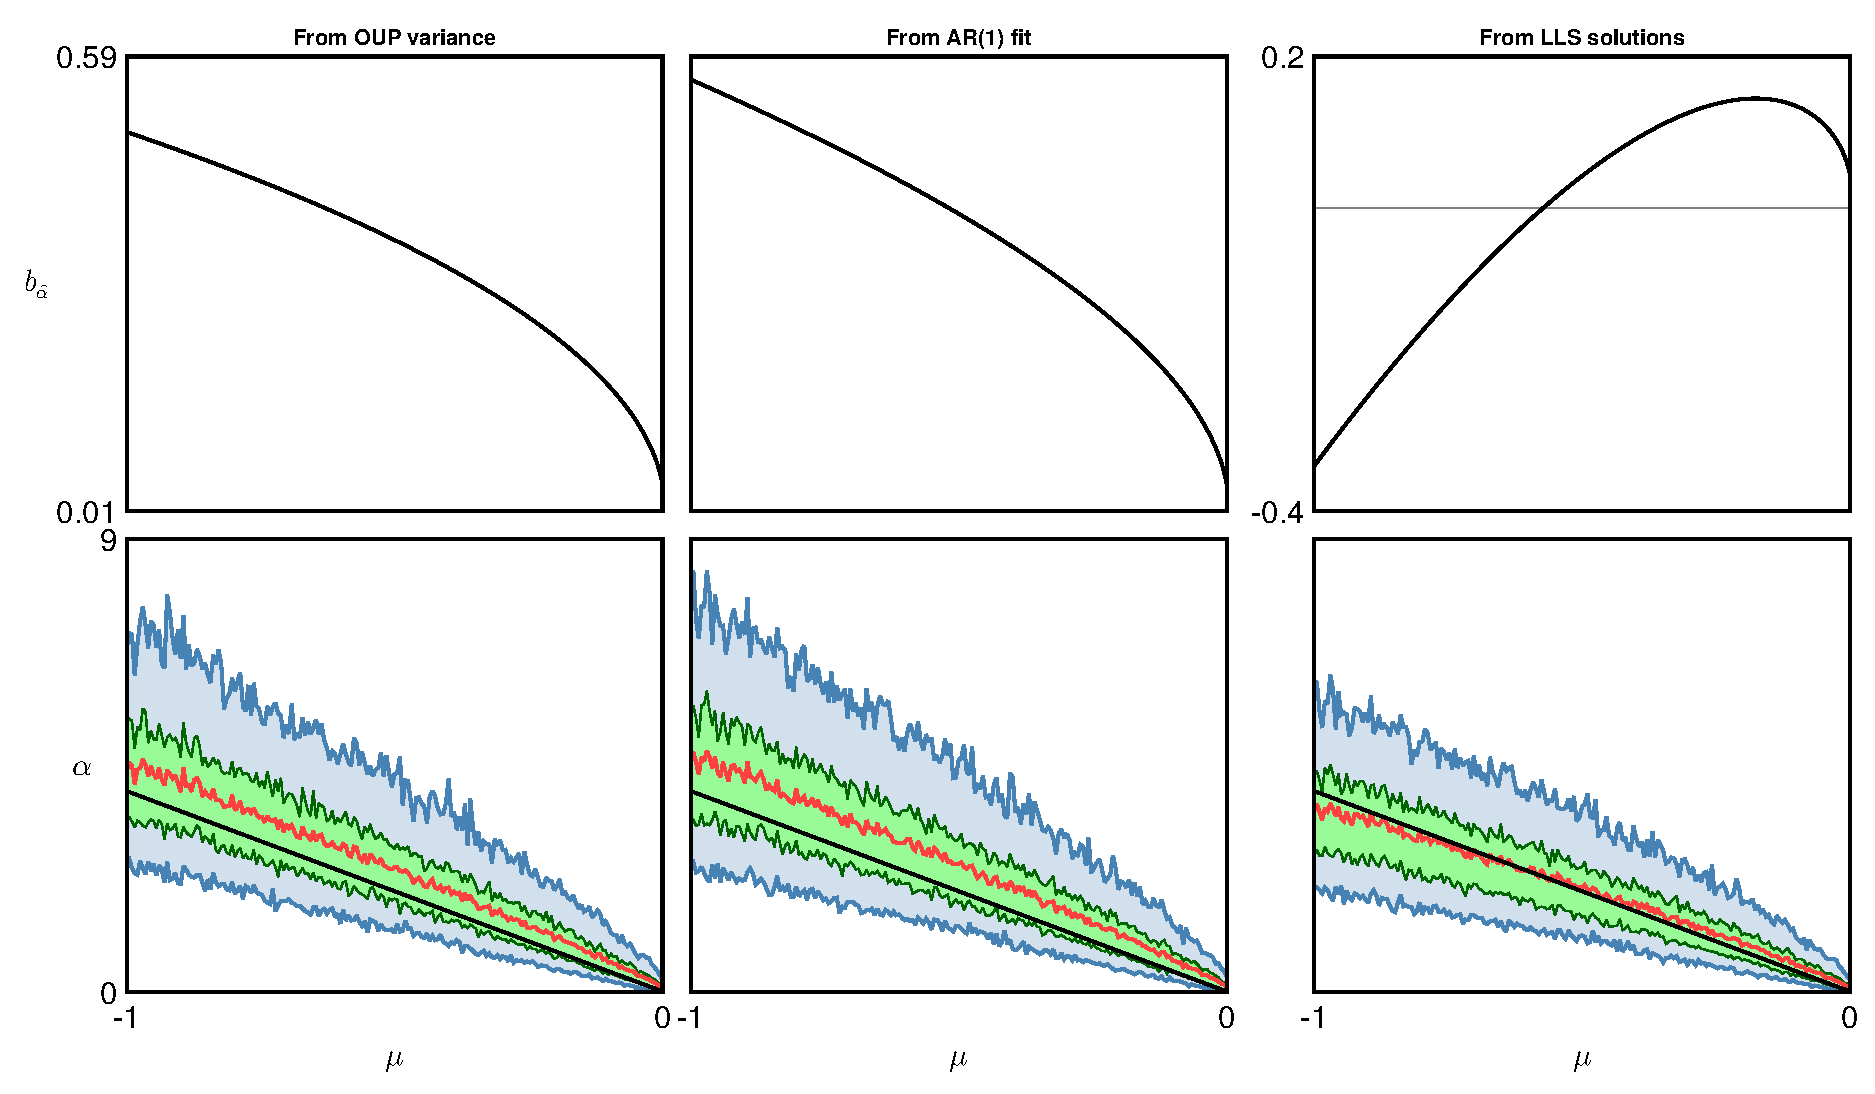
\includegraphics[keepaspectratio, width=\textwidth]{./figures/bias_estimators.pdf}
    \caption{Comparison of the bias of the return rate estimators \eqref{eq:return_rate_bias} (top row) obtained from the sample variance \eqref{eq:OUP} (left), sample autocorrelation \eqref{eq:AC1} (middle) and linear least squares solution \eqref{eq:LLS} (right). Notice how the estimator from the sample variance and autocorrelation are positively biased up to the saddle-node bifurcation, compared to the estimator for the least squares regression which crosses zero (gray horizontal line in the top right) at the parameter value prescribed by \eqref{eq:unbiased_LLS}.
    These results are validated by Monte Carlo simulations (bottom row) in which an ensemble $\Omega$ of $N=200$ particles' trajectories of \eqref{eq:model} are solved at fixed values parameter of $\mu$ in a discretized sweep of $200$ points in $[-1,0)$.
    Each trajectory forms a sample $\mathcal{X}\in\Omega$ of $n=400$ observations of noise intensity $\sigma=0.02$. 
    The estimators $\hat\alpha$ in \eqref{eq:OUP}, \eqref{eq:AC1} and \eqref{eq:LLS} are then computed from the sample $\mathcal{X}$ using the prescribed methodology and the ensemble statistics, such as mean (red curve), interquartile range (green shaded region bounded by dark green curves) and $5^{\text{th}}$-$95^{\text{th}}$ interval (blue shaded region bounded by dark blue curves), are compared with the ground truth $\alpha$.}
    \label{fig:bias_estimators}
\end{figure}

\subsubsection{Optimal observation length}\label{subsubsec:window}
The topic of selecting an optimal window length to forecast critical transitions was addressed in \cite{Chen2022}.
In particular, the authors showed that windowed observations with less than $10\%$ of the data from a given sample yield spurious early-warning signals.
Such study however only considers fixed window lengths across a solution approaching a critical transition, which neglects the changing characteristic of the solution in the slow passage through the saddle-node.
Here we derive the optimal, time-dependent window length of a sample for the accurate forecasting of the tipping time. 

Given a sample $\mathcal{X}=\{X_{t_1},\dots,X_{t_n}\}$ recorded across a window $T_{w}=t_n-t_1$, we look for bounds of the form
%
\begin{equation}\label{eq:bounds}
  L(t)\ll T_\mathrm{w} \ll U(t) ,
\end{equation}
% 
in which the residuals retain the necessary properties for the estimation of the return rate \eqref{eq:return_rate}.
The lower bound $L(t)$ is derived by imposing that the sample $\mathcal{X}$ is observed on a window that is much longer than the relaxation time $1/|\lambda|$ which, from \eqref{eq:eigenvalue_time}, reads
%
\begin{equation}\label{eq:lower_bound}
  L(t) = \frac{1}{2\sqrt{\varepsilon(\tau-t)}}\ll T_{\mathrm{w}}.
\end{equation}
%
This requirement ensures that the realizations $X_j$ in the sample are independent fluctuations around the stable equilibrium $x_+(\mu(t))$.
On the other hand, the upper bound $U(t)$ is derived by imposing that the sample $\mathcal{X}$ is quasi-stationary.
To derive $U(t)$ observe that, from \eqref{eq:eigenvalue_time}, the instantaneous rate of change of the eigenvalue is
%
\begin{equation*}
  \frac{\dd \lambda}{\dd t} \eqqcolon\dot\lambda(t) = \frac{2\varepsilon}{|\lambda(t)|} ,
\end{equation*}
%
which is positive and monotonically increasing for any $t<\tau$, which implies that $\dot\lambda(t_n)=\sup_{t_1<t<t_n}\dot\lambda(t)$ over any finite time window $(t_1,t_n)$.
By setting $T_{w}=t_n-t_1$ it follows
%
\begin{equation*}
  0<\Delta\lambda = \lambda(t_n) - \lambda(t_1) = \int_{t_1}^{t_n}\dot\lambda(t)dt < \dot\lambda(t_n)T_{\mathrm{w}}  = \frac{2 \varepsilon}{|\lambda(t_n)|}T_{\mathrm{w}},
\end{equation*}
%
and dividing each term by $|\lambda(t_n)|$ yields
%
\begin{equation*}
  \frac{\Delta\lambda}{|\lambda(t_n)|} < \frac{2 \varepsilon}{\lambda^2(t_n)}T_{\mathrm{w}} .
\end{equation*}
%
Our requirement for the sample $\mathcal{X}$ to be quasi-stationarity across $T_{w}$ corresponds to small changes of the leading eigenvalue compared to its endpoint value, i.e. $\Delta\lambda/|\lambda(t_n)|\ll 1$, which is guaranteed by imposing
%
\begin{equation*}
  \frac{2 \varepsilon}{\lambda^2(t_n)}T_{\mathrm{w}} \ll 1 ,
\end{equation*}
%
yielding a sufficient condition for the upper bound of the window length
%
\begin{equation}\label{eq:upper_bound}
  T_\mathrm{w}\ll U(t) = \frac{\lambda^2(t)}{2 \varepsilon} = 2(\tau - t),
\end{equation}
%
where the last equality follows from \eqref{eq:return_rate}.
Plugging \eqref{eq:lower_bound} and \eqref{eq:upper_bound} into \eqref{eq:bounds} provides us with the window length protocol
%
\begin{equation}\label{eq:window_length}
  \frac{1}{2\sqrt{\varepsilon(\tau-t)}}\ll T_{\mathrm{w}} \ll 2(\tau - t),
\end{equation}
%
where notice that only the lower bound depends on the speed of the parameter $\varepsilon$.

\subsection{Extrapolating the tipping time}\label{subsec:extrapolators}
Having derived the design conditions for the collection of samples that yield optimal estimators $\hat\alpha$ we are now ready to specify the full data-driven pipeline for the forecasting of the breaking time $\tau_{\mathrm{tip}}$.
As anticipated in \S~\ref{sec:formulation}, given a sequence of estimators $\hat\alpha=\{\hat\alpha_j\}_{j=1,\dots,N}$, the forecasting of $\tau_{\mathrm{tip}}$ is translated into an extrapolation problem $\hat\tau = -\hat q/\hat m$ via the linear fit $\hat\alpha(t)=\hat m t + \hat q$ of slope $\hat m$ and intercept $\hat q$.
As for the Euler--Maruyama approximation outlined in \S~\ref{subsec:LLS}, the linear regression of the sample $\hat\alpha$ to the fit $\hat q,\hat m$ corresponds to a linear least--squares problem whose solution is given by the normal equation 
%
\begin{equation}\label{eq:ordinary_regression}
  \begin{pmatrix}
       \hat q \\
       \hat m
     \end{pmatrix} = \Bigl(B^TB\Bigr)^{-1}B^T\hat\alpha,
\end{equation}
%
where $B = (1, t_j)_{j=1,...,N}$ is the model matrix and $\hat\alpha_j=\hat\alpha(t_j)$ is the estimated return rate at time $t_j$.
To be an efficient estimator of $(\hat q,\hat m)^T$ the solution \eqref{eq:ordinary_regression} requires that the uncertainty in the input data is homogeneous (i.e. assuming \emph{homoskedasticity}) .
This however is clearly not the case for the return rate sample $\hat\alpha$ as evidenced in Figure~\ref{fig:bias_estimators}; in particular, all three estimators \eqref{eq:OUP}, \eqref{eq:AC1} and \eqref{eq:LLS} appear to have decreasing uncertainty as the system is driven closer to the saddle-node bifurcation.
Therefore the heterogeneity in the uncertainty of the sample $\hat\alpha(t)$ (i.e. \emph{heteroskedasticiy}) makes the ordinary least--square regression \eqref{eq:ordinary_regression} an inefficient point estimate of the linear trend $\hat m$ and intercept $\hat q$ \cite{White1980}.
Assuming that, albeit heterogeneous, the uncertainty $u_{\hat\alpha_j}$ in the estimate $\hat\alpha_j$ is uncorrelated with that of any other estimate $\hat \alpha_k$ in the sequence $\hat\alpha$, then the weighted least--square formulation
%
\begin{equation}\label{eq:weighted_regression}
  \begin{pmatrix}
       \hat q \\
       \hat m
     \end{pmatrix} = \Bigl(B^TWB\Bigr)^{-1}B^TW\hat\alpha,\quad W = \mathrm{diag}\Bigl(u^{-2}_{\hat\alpha_j}\Bigr)_{j=1,\dots,N},
\end{equation}
%
provides the best possible (unbiased) estimator for the linear fit \cite{Aitken1936}.
Using the squared residuals of the ordinary least--squares solution \eqref{eq:ordinary_regression} as heteroskedasticiy--consistent estimators of the entries of the weight matrix $W$ \cite[Thm.~$1$]{White1980}, one can thus implement the full, data-driven (weighted) extrapolation problem \eqref{eq:weighted_regression}, from the sequence $\hat\alpha$, to finally forecast the breaking time $\hat\tau$.

\section{Practical applications}\label{sec:application}
The tipping time framework and observation protocal specified in \S~\ref{sec:tipping},\ref{sec:observation} respectively provides us with a series of constraints to collect or generate timeseries samples in order to apply the proposed, data--driven, forecasting pipeline.
These constraints allow for the optimal design of experiments, data collection and modeling choices for applications and are summarized as follows: 
%
\begin{enumerate}
  \item the noisy fluctuations in the residuals $\mathcal{X}$ are additive, i.e. $\sigma(x)=\sigma>0$, and small compared to the timescale separation between the state $x$ and its parameter $\mu$, i.e. $\sigma\ll\sqrt{\varepsilon}$;
  \item the residuals are collected prior to the critical transition and within the admissible time horizon $T_c < \tau - \varepsilon^{-1/3}$;
  \item the residuals are sampled at regular frequency resulting in constant, small enough time intervals $\Delta$ to control bias and uncertainty in the estimation of the return rate $\hat\alpha$;
  \item the residuals are collected over a time window that is long enough so that the correlation in the observation is negligible, i.e. $1/(2\sqrt{\varepsilon(\tau - t)})\ll T_w$, and short enough so that the sample can be considered a stationary approximation of the nonlinear evolution, i.e. $T_w\ll 2(\tau - t)$.
\end{enumerate}
%
We hereby apply this constraints to design the optimal conditions for which data can be collected to accurately forecast the breaking time.

To do so we first consider the canonical case of the dynamic saddle-node normal form \eqref{eq:model} to show how the pipeline performs in the forecast of a simplified model.
We subsequentially apply our methodology to the timeseries data of ... AMOC?

\subsection{Dynamic saddle-node normal form}\label{subsec:dynamic_sn_normal_form}

\subsection{AMOC ?}\label{subsec:amoc}
Edge states for saddle-node escapes in $5-$box model of AMOC \cite{Boers2021,Lohmann2025a}.

\section{Conclusions}\label{sec:conclusion}
So far the theory of early-warning signals has largely been developed within the same setup we considered through this paper: slow, linear passage through saddle-node bifurcations in low-dimensiona, additive noisy systems.
This leaves a large set of models for which the theory has not been developed yet, if not in very incremental steps.
The relaxation of the above assumptions requires extensive mathematical development; recent early development being made in that direction include works on systems driven by multiplicative noise \cite{Morr2024b} and jump processes \cite{Layritz2025}, nonlinear \cite{Ritchie2016} and periodically \cite{Kuehn2018} forced parameter shifts with no timescale separattion, and spatially extended models \cite{Gowda2015,Bernuzzi2024,Clarke2026,Miyauchi2026}.

%%%%%%%%%%%%%%%%%%%%%%%%%%%%%%%%%%%%%%%%%%%%
%               Declarations               % 
%%%%%%%%%%%%%%%%%%%%%%%%%%%%%%%%%%%%%%%%%%%%

\vskip6pt
\enlargethispage{20pt}

\dataccess{The code used to generate the figures is available at the repository \url{https://github.com/papadeiv/Research/tree/master/2027_proc_r_soc_a}.}
\aucontribute{D.P.: Conceptualization, Methodology, Formal analysis, Investigation, Writing - Original draft preparation; L.S.: Supervision, Conceptualization, Validation, Writing - Review \& editing; G.D.: Project administration, Supervision, Funding acquisition, Conceptualization, Validation, Writing - Review \& editing.\\ All authors gave final approval for publication and agreed to be held accountable for the work performed
therein.}
\conflict{We declare we have no competing interests.}
\funding{D.P. and G.D. have received support from the Royal Society of New Zealand, Te Ap\={a}rangi by the Marsden fund n.UOA2223; L.S. has received support from the Royal Society of New Zealand, Te Ap\={a}rangi by the Marsden fund n.23-UOA-152.}
%\ack{We thank the reviewers.}

%%%%%%%%%%%%%%%%%%%%%%%%%%%%%%%%%%%%%%%%
%               Appendix               % 
%%%%%%%%%%%%%%%%%%%%%%%%%%%%%%%%%%%%%%%%

\section*{Appendix A}
\subsection{Something important}

Example table.

\begin{table}[!h]
\caption{An Example of a Table}%%%Table caption goes here
\label{table_example}
\begin{tabular}{llll}%%%The number of columns has to be defined here
\hline
date &Dutch policy &date &European policy \\
\hline
1988 &Memorandum Prevention &1985 &European Directive (85/339) \\
1991--1997 &{\bf Packaging Covenant I} & & \\
1994 &Law Environmental Management &1994 &European Directive (94/62) \\
1997 &Agreement Packaging and Packaging Waste & & \\\hline
\end{tabular}
\vspace*{-4pt}
\end{table}%%%End of the table

%%%%%%%%%%%%%%%%%%%%%%%%%%%%%%%%%%%%%%%%%%%%
%               Bibliography               % 
%%%%%%%%%%%%%%%%%%%%%%%%%%%%%%%%%%%%%%%%%%%%

\vskip2pc

\bibliographystyle{RS}
\bibliography{references}

\end{document}
